% Integration fixture for book structure, environments and references.
% Copyright 2026 Adib Hasan. LPPL 1.3c or later.
\documentclass[12pt,twoside]{bookbangla}
\setbanglamainfont{Kalpurush}
\setmainfont{TeX Gyre Pagella} % Optional: choose an English font.
\title{গণিতের ছোট্ট বই}
\author{আদীব হাসান}
\date{২০২৬}

\begin{document}
\frontmatter
\begin{titlingpage}
\maketitle
\end{titlingpage}
\tableofcontents*
\mainmatter
\chapter{গণনার শুরু}
\begin{chapquote}{লেখক}
ছোট প্রশ্ন থেকেই অনেক বড় ধারণার জন্ম হয়। A small question can open a new door.
\end{chapquote}
\section{পায়রার খোপ নীতি}\label{sec:pigeonhole}
\firstword{আ}{মরা} পরিচিত একটি ধারণা দিয়ে শুরু করি। বাংলা ও English একই
অনুচ্ছেদে লিখলেও প্রতিটি ভাষা তার নিজস্ব ফন্ট রাখে।
\textbf{গুরুত্বপূর্ণ কথা bold করা যায়}, আর \textit{বিশেষ কথায় italic ব্যবহার করা যায়}।%
\footnote{এই বইয়ের উদাহরণগুলো নিজে চেষ্টা করে দেখো।}

\begin{theorem}[পায়রার খোপ নীতি]
$n+1$টি বস্তু $n$টি খোপে রাখলে অন্তত একটি খোপে দুটি বস্তু থাকবে।
\end{theorem}
\begin{proof}
প্রতি খোপে সর্বোচ্চ একটি বস্তু থাকলে মোট বস্তুর সংখ্যা $n$-এর বেশি হতে পারে না।
\end{proof}
\begin{example}[label=example:weekdays]
আটজন বন্ধুর মধ্যে অন্তত দুজনের জন্ম একই বারে কেন?
\end{example}
\begin{solution}
সপ্তাহের সাতটি বারকে খোপ এবং আটজন বন্ধুকে বস্তু হিসেবে ধরলেই হয়।
\end{solution}
\begin{remark}
এখানে জন্মসাল জানার প্রয়োজন নেই।
\end{remark}
\begin{reminder}
বস্তু ও খোপ ঠিকভাবে চিহ্নিত করাই এই নীতির প্রধান ধাপ।
\end{reminder}
\begin{diybox}
\begin{smartlist}
\item দশজন বন্ধুর জন্য একই যুক্তি ব্যবহার করো।
\item খোপের সংখ্যা বাড়ালে কী পরিবর্তন হয়?
\end{smartlist}
\end{diybox}

\section{অনুশীলনী}
\begin{exercise}[hint={বছরের মাসগুলোকে খোপ ধরো; $13>12$।}]
\label{exercise:months}
তেরোজন মানুষের মধ্যে অন্তত দুজনের জন্ম একই মাসে, দেখাও।
\end{exercise}
\begin{exercise}\label{exercise:remainders}
চারটি পূর্ণসংখ্যার মধ্যে অন্তত দুটির $3$ দিয়ে ভাগশেষ সমান, দেখাও।
\end{exercise}
\section{আরও অনুশীলনী}
\begin{exercise}\label{exercise:continued}
আগের সমস্যায় চারটির পরিবর্তে সাতটি সংখ্যা নিলে কী বলা যায়?
\end{exercise}
\autoref{exercise:months} এবং \autoref{example:weekdays}-এ একই ধারণা আছে।
\autoref{sec:pigeonhole}-এ নীতিটি বলা হয়েছে।

\chapter{যোগফল ও চিত্র}
\section{একটি পরিচিত যোগফল}
\begin{example}\label{example:sum}
প্রথম $n$টি ধনাত্মক পূর্ণসংখ্যার যোগফল নির্ণয় করো।
\end{example}
\begin{equation}\label{eq:sum}
  \underbrace{1+2+\cdots+n}_{\text{প্রথম }n\text{টি সংখ্যা}}
  = \frac{n(n+1)}{2}.
\end{equation}
সমীকরণ~\eqref{eq:sum} থেকে $n=৫$ বসিয়ে যোগফল $১৫$ পাওয়া যায়।
\begin{exercise}[hint={দুটি সমান যোগফল বিপরীত ক্রমে সাজাও।}]
\label{exercise:newchapter}
যোগফলের সূত্রটি প্রমাণ করো।
\end{exercise}

\begin{table}[htbp]
\centering
\begin{tabular}{lr}
\toprule
বস্তুর সংখ্যা & খোপের সংখ্যা\\
\midrule
৮ & ৭\\
১৩ & ১২\footnote{এখানে মাসের সংখ্যা ব্যবহার করা হয়েছে।}\\
\bottomrule
\end{tabular}
\caption{উদাহরণের বস্তু ও খোপ}\label{table:boxes}
\end{table}
\begin{figure}[htbp]
\centering
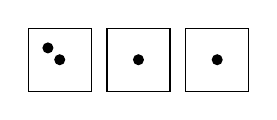
\begin{tikzpicture}
\foreach \x in {0,1,2} {
  \draw (\x,0) rectangle +(0.8,0.8);
  \fill (\x+0.4,0.4) circle (2pt);
}
\fill (0.25,0.55) circle (2pt);
\end{tikzpicture}
\caption{তিনটি খোপে চারটি বস্তু}\label{figure:boxes}
\end{figure}
\autoref{table:boxes} এবং \autoref{figure:boxes} ধারণাটি দেখায়।
আরও আলোচনার জন্য দেখো~\cite{graham}।

\appendix
\chapter{কিছু নির্দেশনা}
সমস্যা পড়ে আগে নিজে চেষ্টা করো, তারপর ইঙ্গিত দেখো।
\begin{exercise}\label{exercise:appendix}
তোমার নিজের একটি পায়রার খোপ নীতির সমস্যা তৈরি করো।
\end{exercise}
\backmatter
\begin{thebibliography}{9}
\bibitem{graham} Ronald L. Graham, Donald E. Knuth and Oren Patashnik,
\emph{Concrete Mathematics}, second edition, Addison-Wesley, 1994.
\end{thebibliography}
\end{document}
